%\documentclass[a4paper,10pt]{report}
\documentclass{report}
\usepackage[utf8x]{inputenc}    
\usepackage[T1]{fontenc}
\usepackage[francais]{babel}     
\usepackage{verbatim}
\usepackage{graphicx}
\usepackage{float}
\usepackage{makeidx}
\usepackage{moreverb}
\usepackage{listings}
\usepackage{color}
\usepackage{xcolor}
\usepackage{hyperref}
\usepackage[top=2.5cm,bottom=2.5cm,right=2.5cm,left=2.5cm]{geometry}
\usepackage{here}

\definecolor{mygreen}{rgb}{0,0.6,0}
\definecolor{mygray}{rgb}{0.5,0.5,0.5}
\definecolor{mymauve}{rgb}{0.58,0,0.82}

\lstset{ %
   backgroundcolor=\color{white},   % choose the background color; you must add \usepackage{color} or \usepackage{xcolor}
   basicstyle=\footnotesize,        % the size of the fonts that are used for the code
   breakatwhitespace=false,         % sets if automatic breaks should only happen at whitespace
   breaklines=true,                 % sets automatic line breaking
   captionpos=b,                    % sets the caption-position to bottom
   commentstyle=\color{mygreen},    % comment style
   deletekeywords={...},            % if you want to delete keywords from the given language
   escapeinside={\%*}{*//)},          % if you want to add LaTeX within your code
   extendedchars=true,              % lets you use non-ASCII characters; for 8-bits encodings only, does not work with UTF-8
   frame=single,                    % adds a frame around the code
   keepspaces=true,                 % keeps spaces in text, useful for keeping indentation of code (possibly needs columns=flexible)
   keywordstyle=\color{blue},       % keyword style
   language=Octave,                 % the language of the code
   morekeywords={*,...},            % if you want to add more keywords to the set
   numbers=left,                    % where to put the line-numbers; possible values are (none, left, right)
   numbersep=5pt,                   % how far the line-numbers are from the code
   numberstyle=\tiny\color{mygray}, % the style that is used for the line-numbers
   rulecolor=\color{black},         % if not set, the frame-color may be changed on line-breaks within not-black text (e.g. comments (green here))
   showspaces=false,                % show spaces everywhere adding particular underscores; it overrides 'showstringspaces'
   showstringspaces=false,          % underline spaces within strings only
   showtabs=false,                  % show tabs within strings adding particular underscores
   stepnumber=2,                    % the step between two line-numbers. If it's 1, each line will be numbered
   stringstyle=\color{mymauve},     % string literal style
   tabsize=2,                       % sets default tabsize to 2 spaces
   title=\lstname,                   % show the filename of files included with \lstinputlisting; also try caption instead of title
   language=java
}
\lstset{language=java,caption={Projet A13 LO43}}

\hypersetup{
     bookmarks=true,         % show bookmarks bar?
     unicode=true,          % non-Latin characters in Acrobat’s bookmarks
     pdftoolbar=true,        % show Acrobat’s toolbar?
     pdfmenubar=true,        % show Acrobat’s menu?
     pdffitwindow=false,     % window fit to page when opened
     pdfstartview={FitH},    % fits the width of the page to the window
     pdftitle={Projet LO43},    % title
     pdfauthor={Yoann CAPLAIN},     % author
     pdfsubject={Ticket To UTBM},   % subject of the document
     pdfcreator={Yoann CAPLAIN},   % creator of the document
     pdfproducer={Producer}, % producer of the document
     pdfkeywords={LO43} {CAPLAIN} {A13}, % list of keywords
     pdfnewwindow=true,      % links in new window
     colorlinks=true,       % false: boxed links; true: colored links
     linkcolor=black,          % color of internal links (change box color with linkbordercolor)
     citecolor=green,        % color of links to bibliography
     filecolor=magenta,      % color of file links
     urlcolor=cyan           % color of external links
}
\floatplacement{figure}{t}

\begin{document}
\begin{figure}[!p!t]
%\flushright
%\floatplacement{figure}{t}

\includegraphics[height=60pt]{utbm.png}
\end{figure}

\title{Projet LO43\\ \huge{\textbf{Ticket To UTBM}}}
\author{Yoann \bsc{Caplain}}
\date{\today \\Semestre A2013}



\maketitle \clearpage
\tableofcontents %\clearpage

%\part{Partie}
\chapter{Introduction}
Dans  le  cadre  de  l’unité  de  valeur  “LO43  : les  Bases de  la Programmation Orientée  Objet”,  il   nous  est  demandé  de  réaliser  un  projet  permettant d’appliquer  les  différents  concepts  étudiés  tout  au  long  des  cours,  travaux pratiques et travaux dirigés.
Le projet “Ticket to ride” qui nous a été soumis permet de mettre en oeuvre ces concepts.
%Dans  la  suite  de  ce  document  nous  décriront  toutes  les  démarches  ayant mené à la  réalisation de ce projet, ensuite nous décriront les différentes actions d’un point de vue général que doit effectuer le système en interaction avec l’utilisateur, et, enfin les classes (objets) et la manière dont elles communiquent entre elles.

\section{Rappel du sujet : Ticket To UTBM}
Le  but  du  projet  est  de  réaliser  une  application fonctionnelle en suivant toutes les étapes de  construction d’un projet à partir d’un cahier de charges définissant  la  structure  générale du  système et les scénarios d’utilisations possibles. La  modélisation  de  l’application se fera en  utilisant l'UML et la réalisation devra s’effectuer en JAVA.\\
L'objectif du projet est d'adapter le jeu "ticket to ride" au monde de l'UTBM. Par exemple, chaque tronçon de rail peut correspondre à l'obtention d'une UV. Chaque ville peut correspondre à une catégorie d'UV (TM, CG,...) pour gagner il faut obtenir son diplôme d'ingénieur et donc avoir le plus grand nombre de crédit possible (points), les challenges de ticket to ride correspondent à la jonction entre deux catégories d'UV.\\
Il nous est demandé de concevoir ce jeu en faisant une analyse  UML  du projet en utilisant les  diagrammes nécessaires et ensuite de proposer une implémentation.

\section{Les fonctionnalités du jeu}
Ticket To UTBM a été basé sur le Ticket To Ride existant sur IOS, voici  les fonctionnalités du jeu :
\begin{itemize}
\item Jouer en solo avec des IA
\item Jouer en multi en réseau (avec ou sans IA)
\item Jouer en multi sur le même ordinateur (avec ou sans IA)
\item Sauvegarder une partie et la charger plus tard (utilisation de la serialisation)
\item Changer les options du jeu (musiques, pseudo, résolution, plein écran,...)
\end{itemize}

\chapter{Analyse et conception}
\section{UML : Langage de modélisation}
L'analyse d'un projet est primordiale, ça permet de clarifier les aspects techniques et ce que l'on veut faire sur notre projet. C'est pourquoi cette analyse est très importante et qu'il faut qu'elle soit correct avant le début de la conception du projet car selon l'erreur d'analyse celle-ci peut soit être résolu avec quelques modifications ou nécessite de recommencer la conception du projet.\\


L'analyse qui a été faite sur le projet Ticket To UTBM était correct dès le début, ainsi le projet a pu être programmer sans avoir à repasser par l'analyse du projet.\\
De plus cette analyse a été faite de façons à avoir un code modulable grâce aux factory et la représentation d'une Partie avec ce qui la compose. Et une abstraction totale de l'interface, du rendu pour les joueurs (render()), ce qui permet d'avoir un modèle MVC  simple et efficace avec des pattern tel que :
\begin{itemize}
\item Factory Pattern
\item Game State Pattern (implique forcément le MVC)
\item Singleton Pattern
\end{itemize}
\subsection{Le diagramme de classes}
Ce fût ce qui a été fais en premier puis le jeu a été codé.\\
C'est grâce à ce diagramme que le jeu est modulable, ainsi des factory ont pû être établis et le Game State Pattern utilisé correctement.
\subsubsection{Diagramme de Partie}
\begin{figure}[H]
\center
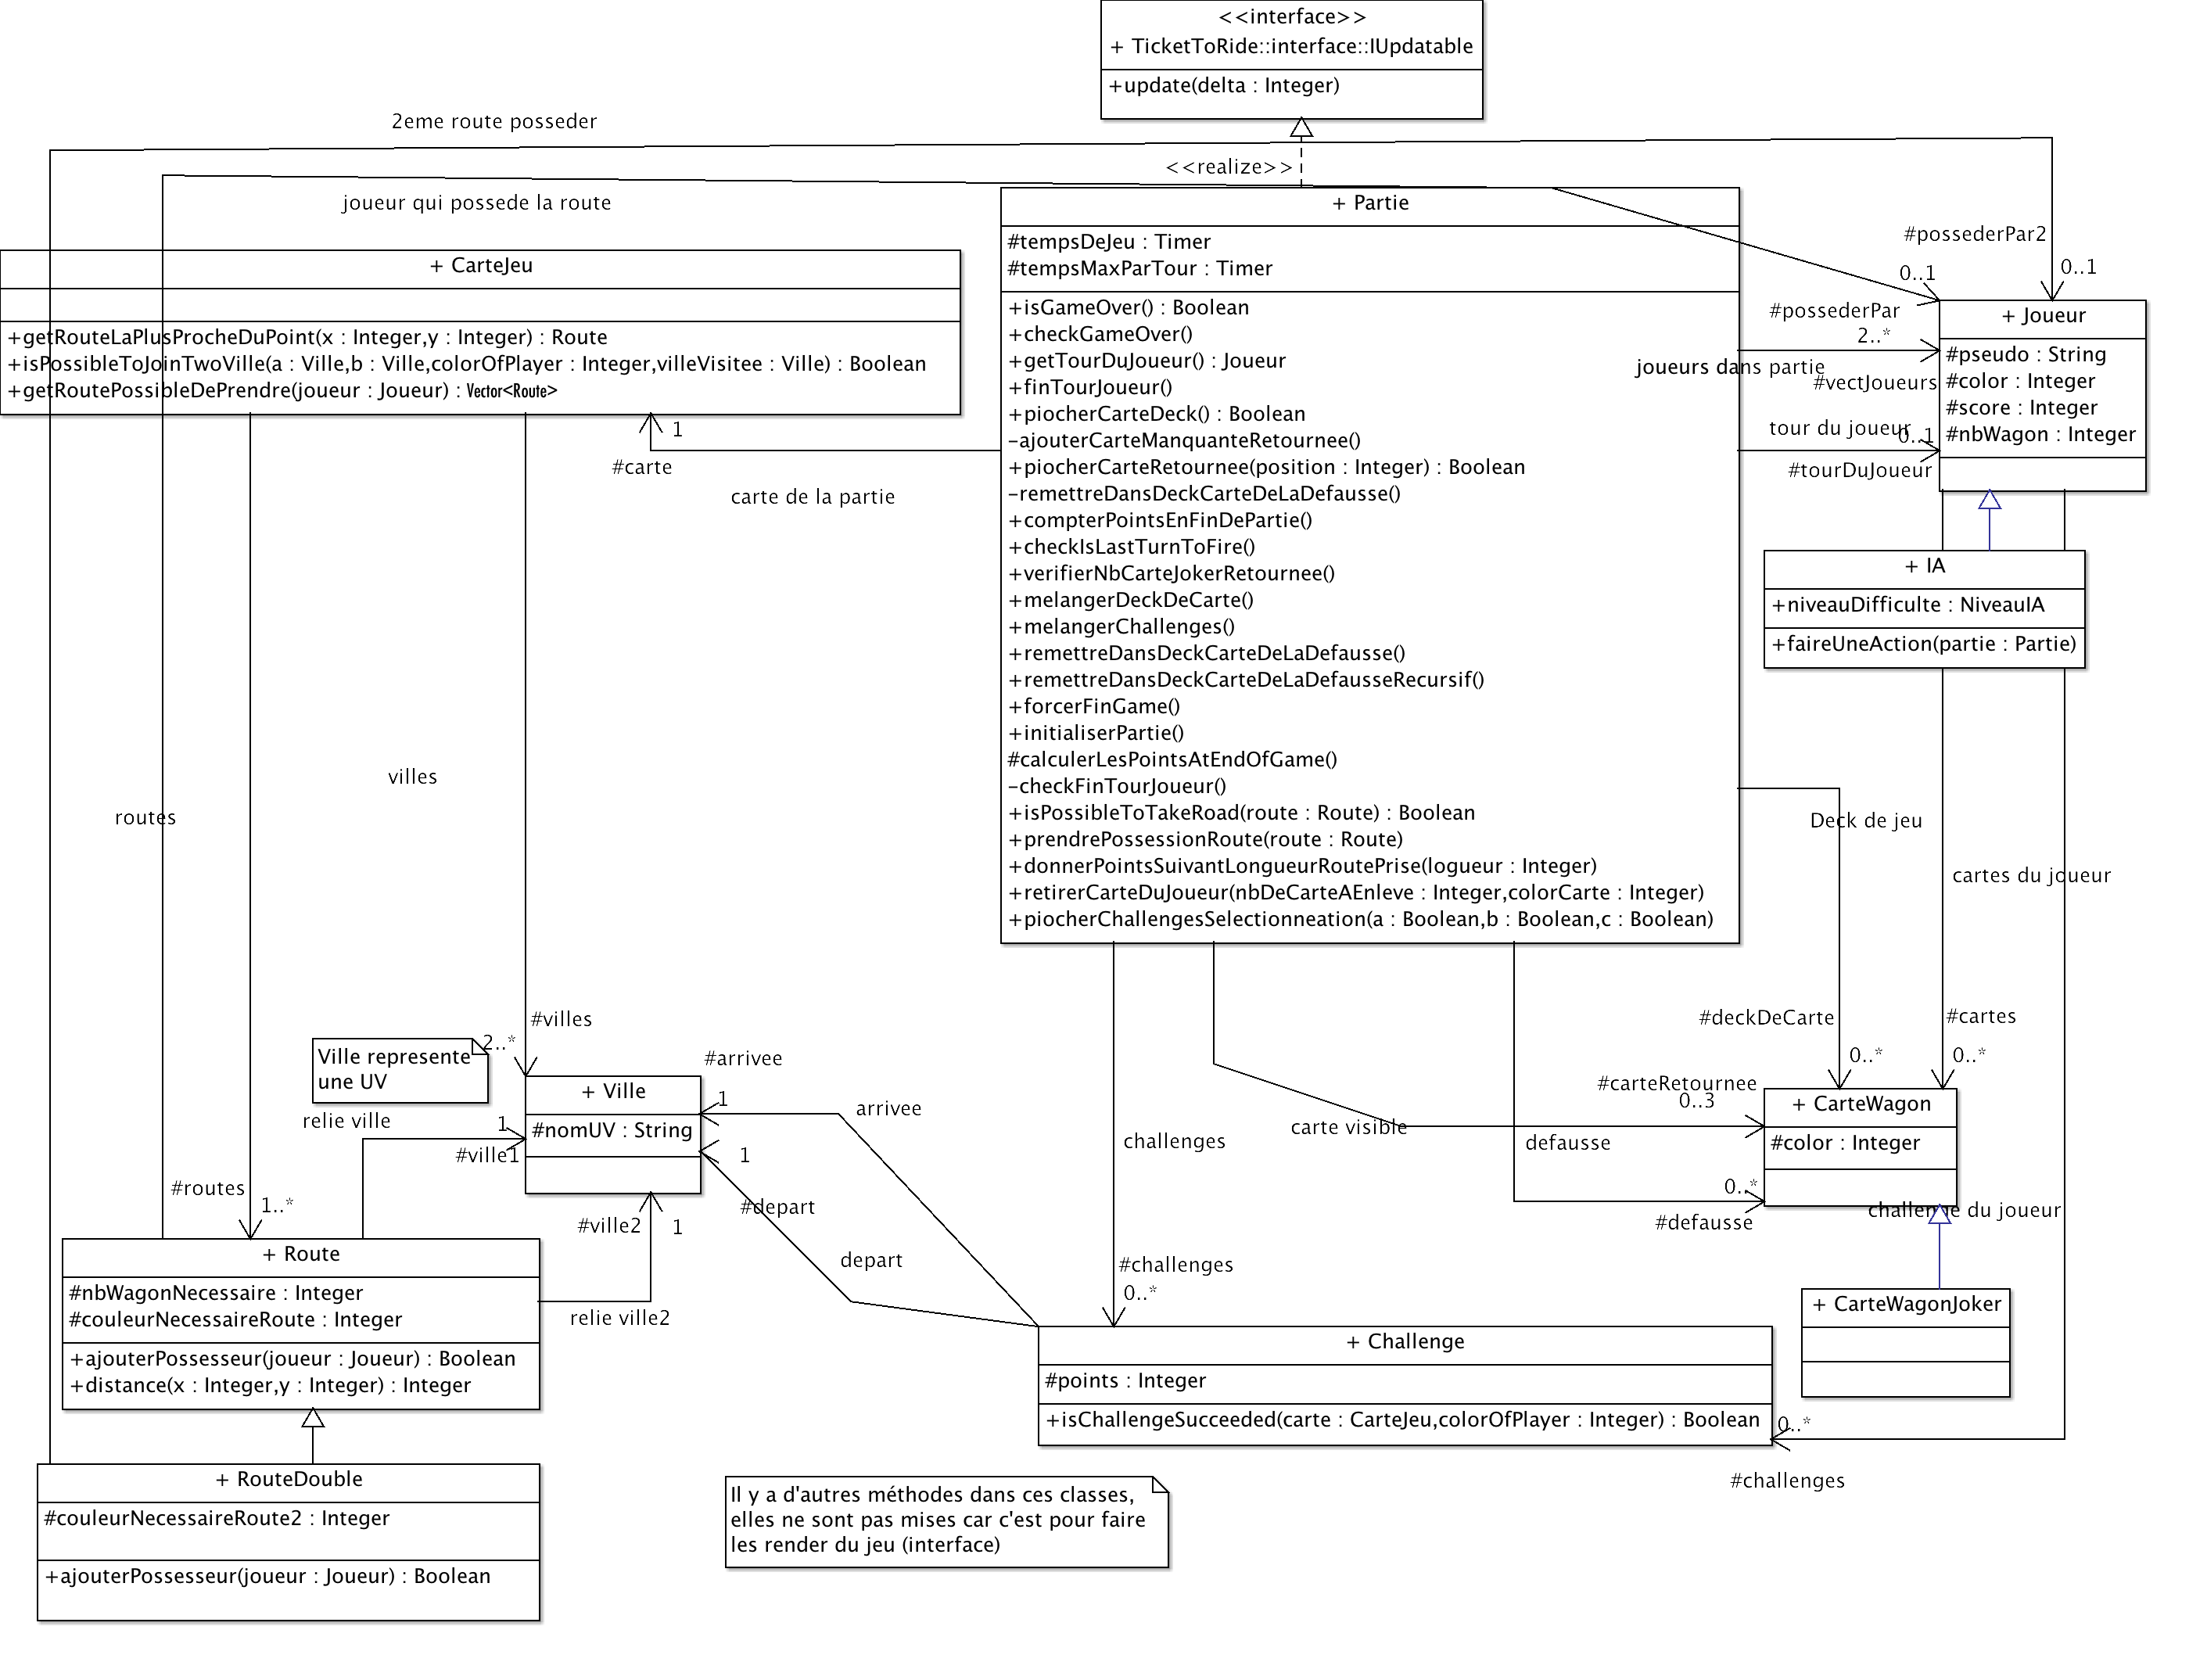
\includegraphics[angle=90,width=500pt]{diagPartie.png}
\caption{Diagramme de Partie}
\label{Diagramme de Partie}
\end{figure}
\subsubsection{Diagramme des factory}
Pour le diagramme de classes des Factory cf chapitre \ref{Factory} page \pageref{Factory}.
\subsubsection{Des diagrammes plus simple}
Voici des diagrammes de classes plus simples mais qui représentent un plus grand ensemble du projet.\\
(cf Annexe \ref{Diagrammes} page \pageref{Diagrammes})

%\subsection{Le modèle fonctionnel}
\subsection{Le diagramme des cas d'utilisation}
Il  montre  le  fonctionnement  du  système  selon  le  point  de  vue  des utilisateurs.  Il  permet  en  d’autres  termes,  d'identifier  les  possibilités d'interaction  entre  le  système  et  les  acteurs.\\
Voici  le  diagramme  des  cas d’utilisation du jeu.
\begin{figure}[H]
\center
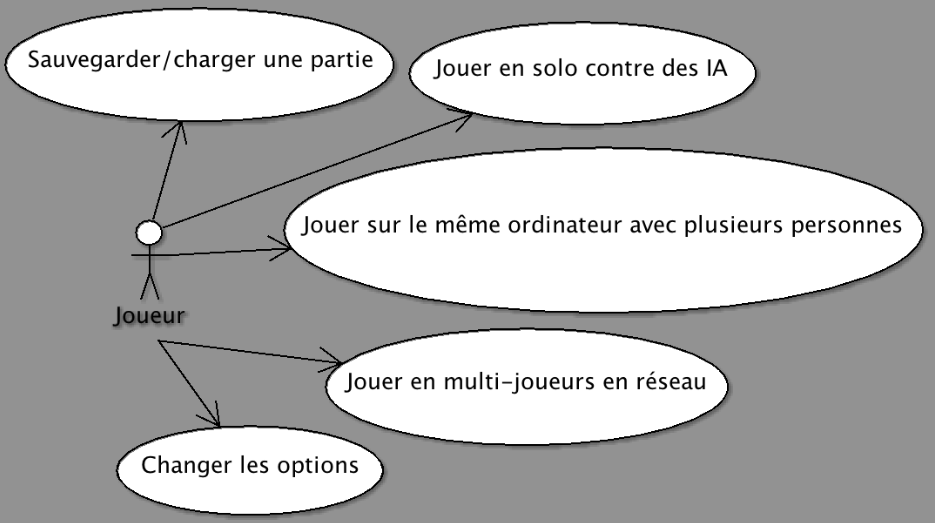
\includegraphics[width=500pt]{casUtilisation.png}
\caption{Diagramme des cas d'utilisations}
\label{Diagramme des cas d'utilisations}
\end{figure}
\newpage
\subsection{Le diagramme de séquence}
Le diagramme de séquence montre ce qui se passe suivant les actions du joueur lors d'une partie.
\begin{figure}[H]
\center
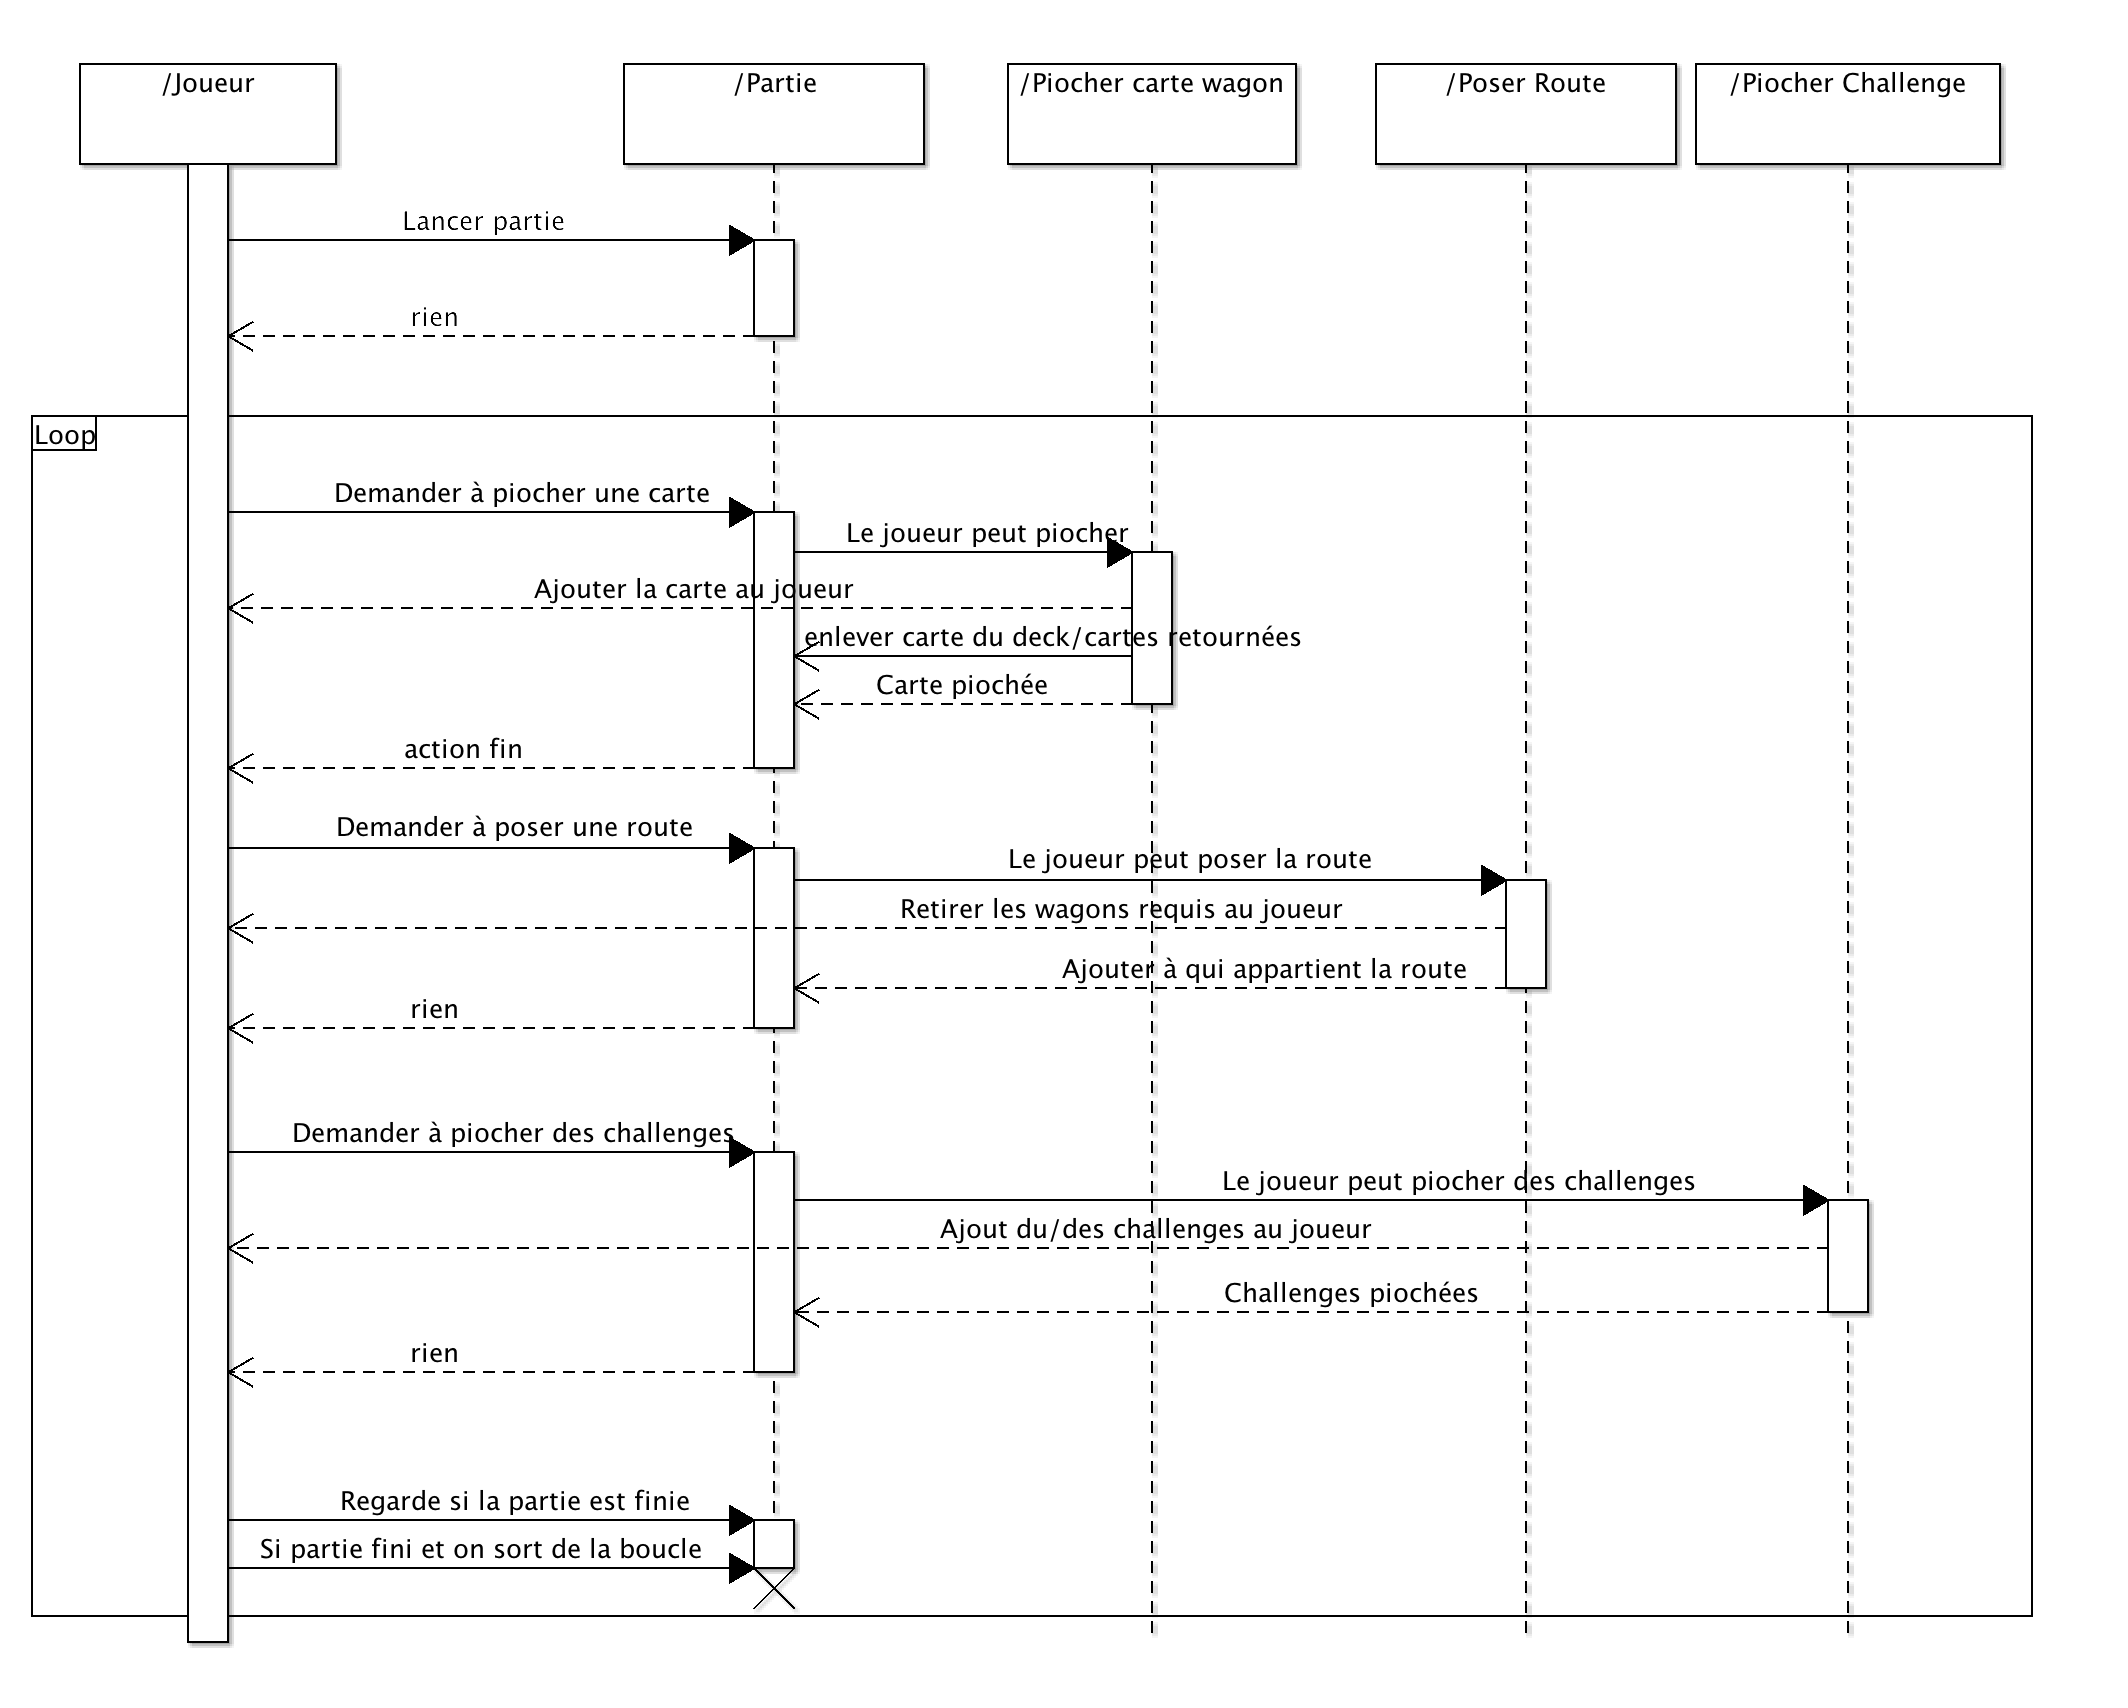
\includegraphics[width=500pt]{diagSeq.png}
\caption{Diagramme de séquence}
\label{diagSeq}
\end{figure}
%\subsection{Le diagramme d'objet}


\chapter{Réalisation du projet}
Le programme utilise la bibliothèque Slick2D qui apporte les éléments nécessaires à l'élaboration de la fenêtre graphique ainsi que des événements (clavier et souris).\\
Son principe de fonctionnement est explicité dans le chapitre \ref{slick2dd} page \pageref{slick2dd}.
\section{Structure générale}
Le projet a été pensé et fais de sorte à respecter un maximum le modèle MVC.\\
Le principe est : les joueurs sont devant leurs vues et selon leurs actions ils déclenchent des interactions avec les controlleurs puis les modèles.
\section{Description des classes}
\subsection{Ville (UV)} \label{defUV}
Un ville représente une UV, l'attribut principale est bien sûr le nom de l'UV. Il a fallu ajouter les positions X et Y pour afficher l'UV correctement sur l'interface du joueur, de plus ces positions servent dans les calculs pour afficher les routes et pour simuler le clique sur une route (prendre possession d'une route). Cf \ref{defRoute} page \pageref{defRoute}
\begin{lstlisting}[caption=Représentation d'une UV]
public class Ville implements IRenderable, IPosition, Serializable{
	private static final long serialVersionUID = -2973170336488215261L;
	protected int x,y; // ajouter du au fait qu'il faut representer une UV a un endroit sur la carte
  protected String nomUV;

  /* Constructeurs... */
	@Override
	public void render(Graphics g,final int deltaX,final int deltaY) {
		// Voir Ville.java
	}
@Override
	public boolean equals(Object a){
		if(a instanceof Ville)
			if(nomUV.equalsIgnoreCase(((Ville)a).nomUV))
				return true;
		return false;
	}
}
\end{lstlisting}
\subsection{Route (et double)} \label{defRoute}
Une route est ce qui relie deux villes (UV), on ne peut prendre une route qu'en ayant un certain nombre de wagon et d'une couleur précise.\\
RouteDouble hérite de Route et redéfinie certaines méthodes de la classe mère telle que render, ajouterPossesseur, etc.\\
L'ajout d'un possesseur de la route se fait seulement si la route n'est pas déjà possedée. Pour la route double l'ajout appel d'abord l'ajout mère, si elle retourne False alors l'ajout est testé sur la 2ème route.


Le joueur peut s'emparer d'une route sur le plateau en posant autant de cartes Wagon de la couleur de la route que d’espaces composant la route (nbWagonNecessaire). Après avoir défaussé ses cartes, le joueur pose alors ses wagons sur chaque espace constituant la route. Et il obtient les points correspondant à l'obtention de la route.
\begin{lstlisting}[caption=Représentation d'une route]
public class Route implements IRenderable, Serializable{
	private static final long serialVersionUID = -6066784805826120870L;
	protected static final int WIDTH_MIN_ROUTE = 10; // pour render
	protected static final int WIDTH_MAX_ROUTE = 30; // pour render

	protected int nbWagonNecessaire;
	protected int couleurNecessaireRoute;
	protected Joueur possederPar;
	protected Ville ville1;
	protected Ville ville2;
	
	/* Constructeurs... */
	@Override
	public void render(Graphics g,final int deltaX,final int deltaY) {
		// Voir Route.java
	}
	protected final int calculerLongueurDesRectangles(){
		int hypo = (int)Math.hypot(ville1.getX()-ville2.getX(),ville1.getY()-ville2.getY());
		return hypo / nbWagonNecessaire;
	}
	protected final float calculerAngleEntreDeuxVilles(){
		// Voir Route.java
	}
	public boolean ajouterPossesseur(Joueur joueur) {
		if(possederPar == null){
			possederPar = joueur;
			return true;
		}
		return false;
	}
	
	/**
	 * Retourne la distance du point (x,y) par rapport a la Line de cette route
	 * Get the shortest distance from a point to this line
	 * @param x
	 * @param y
	 * @return The distance from the line to the point
	 */
	public float distance(final int x,final int y){
		return (new Line(ville1.x,ville1.y,ville2.x,ville2.y)).distance(new Vector2f(x,y));
	}

	/**
	 * On ne verifie pas la personne qui possede la route
	 */
	@Override
	public boolean equals(Object route){
		if(route instanceof Route){
			if(nbWagonNecessaire== ((Route)route).nbWagonNecessaire &&
			couleurNecessaireRoute == ((Route)route).couleurNecessaireRoute &&
			ville1 == ((Route)route).ville1 &&
			ville2 == ((Route)route).ville2)
				return true;
		}
		return false;
	}
}
\end{lstlisting}
\subsection{Challenge} \label{defChallenge}
Chaque carte Challenge fait référence à deux villes (UV) de la carte et un nombre de points y est associé. Si le joueur réalise la connexion entre les deux villes (UV) d’une carte Challenge, il remporte le nombre de points indiqué sur la carte et l’additionne, en fin de partie, aux points déjà acquis.\\
La route reliant ces deux villes (UV) doit être formée uniquement par les trains de ce joueur. Si la connexion n’est pas réalisée, le joueur déduit de son nombre de points déjà acquis le nombre indiqué sur la carte.\\
Les cartes Challenge sont gardées secrètes tout au long de la partie. Elles sont rendues publiques à la fin de la partie et chaque joueur calcule son score. Au cours du jeu, un joueur peut avoir autant de cartes Challenge qu’il le souhaite.
\begin{lstlisting}[caption=Représentation d'un challenge]
public class Challenge implements Serializable{
	private static final long serialVersionUID = -2546823565778080558L;

	protected int points;
	protected Ville arrivee; // UV
	protected Ville depart; // UV
	
	/* Constructeurs... */
/**
	 * @param carte la carte qui contient les villes et routes
	 * @param colorOfPlayer couleur du joueur
	 * @return true si reussi
	 */
	public boolean isChallengeSucceeded(final CarteJeu carte, final int colorOfPlayer){
		return carte.isPossibleToJoinTwoVille(depart, arrivee, colorOfPlayer,null);
	}
}
\end{lstlisting}
\subsection{CarteWagon et Joker} \label{defCarteWagon}
Une carte wagon est une carte qui a une couleur, cette couleur sert à prendre les routes qui ont la même couleur.
\begin{lstlisting}[caption=Représentation d'une carte]
public class CarteWagon implements Serializable{
	private static final long serialVersionUID = 2206179139888856797L;
	protected int color;

  /* Constructeurs... */
}
\end{lstlisting}


La carte Joker est une carte spéciale qui permet de remplacer n'importe quel couleur. Elle permet donc de prendre des routes où le joueur n'a pas assez de la couleur demandée.%, ce qui signifie que les cartes joker permettent de remplacé les cartes manquantes pour prendre possession d'une route.
\begin{lstlisting}[caption=Représentation d'une carte Joker]
public class CarteWagonJoker extends CarteWagon {
	private static final long serialVersionUID = 3393642683536023035L;

	public CarteWagonJoker(){
		super.color = Colors.GRIS;
	}
}
\end{lstlisting}

\subsection{CarteJeu} \label{defCarteJeu}
La classe CarteJeu contient l'ensemble des UV et routes de la partie.\\
On peut voir que la méthode render implementée par IRenderable appelle le render des routes et des villes, ainsi la carte de jeu est affichée.\\
La méthode getRouteLaPlusProcheDuPoint permet de rechercher la route la plus proche du point aux coordonnées (x,y).
\begin{lstlisting}[caption=Représentation d'une carte de jeu]
public class CarteJeu implements IRenderable, Serializable{
	private static final long serialVersionUID = -1724428464393291062L;
	protected Vector<Ville>  villes = new Vector<Ville>();
	protected Vector<Route>  routes = new Vector<Route>();
	/* Constructeurs... */
	@Override
	public void render(Graphics g,final int deltaX,final int deltaY) {
		for(Route v : routes)
			if(v != null)
				v.render(g, deltaX, deltaY);
		for(Ville v : villes)
			if(v != null)
				v.render(g, deltaX, deltaY);
	}
	/**
	 * Retourne la route la plus proche du x,y
	 * @return a copy sinon null si distance superieur a 30.0f
	 */
	synchronized public Route getRouteLaPlusProcheDuPoint(final int x,final int y){
		float min=9999999.0f, calc = 999999.0f;
		Route tmp = null;
		for(Route v : routes){
			if(v != null){
				calc = v.distance(x, y);
				if(calc < min && calc < 30.0f){
					min = calc;
					tmp=v;
				}
			}
		}
		return tmp;
	}
}
\end{lstlisting}
\subsection{Joueur} \label{defJoueur}
Un joueur a un pseudo, une couleur unique qui joue le rôle d'identifiant, des wagons pour prendre possession de route, et un booléen pour savoir si ce joueur est une IA ou une personne.\\
Les Vector challenges et cartes sont respectivement les cartes challenges et les cartes wagon que le joueur possède.
\begin{lstlisting}[caption=Représentation d'un joueur]
public class Joueur implements Serializable{
	private static final long serialVersionUID = 1222L;
	protected String pseudo;
	/**
	 * Unique par joueur (comme un id)
	 */
	protected int color;
	protected int score;
	protected int nbWagon = Regles.NB_WAGON_PAR_JOUEUR;
	protected boolean isIA;

	protected Vector<Challenge>  challenges = new Vector<Challenge>();
	protected Vector<CarteWagon>  cartes = new Vector<CarteWagon>();

	/* Constructeurs... */ 
	synchronized public int compterNbCarteDeTelleCouleur(int color){
		int somme=0;
		for(int i=0;i<cartes.size();++i)
			if(cartes.get(i).getColor() == color)
				somme +=1;
		return somme;
	}
	@Override
	synchronized public boolean equals(Object a){
		if(a instanceof Joueur)
			return ((Joueur)a).color == color;
		return false;
	}
}
\end{lstlisting}
\subsection{Partie} \label{defPartie}
C'est la classe principale d'une partie c'est là que sont regroupées toutes les méthodes qui vont être utilisées dans une partie telle que:
\begin{itemize}
\item Piocher une carte du deck ou de celles retournées
\item Piocher des cartes challenges
\item Demander à prendre possession d'une route
\item Exécuter la fin d'un tour
\item Ajouter les points lors de la prise d'une route
\item Initialiser une partie
\item Déclencher la fin d'une partie
\item etc
\end{itemize}
Voir la classe Partie.java (trop de ligne pour mettre dans le rapport) donc ce qui suit n'est que la déclaration des attributs.
\begin{lstlisting}[caption=Les attributs d'une partie]
public class Partie implements IUpdatable, Serializable {
	private static final long serialVersionUID = -4317180942233324696L;
	
	private static final int TEMPS_MAX_PAR_TOUR = 50000; // 50 secondes
	protected Timer tempsDeJeu, tempsMaxParTour;

  protected Vector<Challenge>  challenges;
  protected CarteJeu carte;
  protected Vector<Joueur>  vectJoueurs;
  protected Vector<CarteWagon>  deckDeCarte;
  protected Vector<CarteWagon>  defausse;
  protected Vector<CarteWagon> carteRetournee;
  protected Joueur tourDuJoueur;

  protected boolean lastTurn;
  protected boolean gameIsOver;
  
  /*
   * Possibilites lors d'un tour
   */
  /** Max 2 */
  protected int compteurCarteDeckPiocher = 0;
  /** Max 2 */
  protected int compteurCarteRetourneePiocher = 0;
  protected boolean carteChallengesPiocher = false;
  protected boolean routePoser = false;
// ...
}
\end{lstlisting}

\subsection{La sauvegarde/chargement}
Permettre la sauvegarde et le chargement d'une partie fût simple à implémenté puisqu'il a suffit d'ajouter l'interface Serializable aux classes de la partie (Partie, Joueur, etc)\\
La classe Sauvegarde permet de faciliter la sauvegarde de tout objet qui implemente l'interface Serializable.
\lstinputlisting[language=java, firstline=9, lastline=50,caption=Classe Sauvegarde]{../src/lo43_TicketToRide/utils/Sauvegarde.java}

\begin{lstlisting}[caption=Sauvegarder une partie (classe PartieView)]
if(rectSave.contains(x, y))
				if(!textSave.getText().equalsIgnoreCase(""))
					if(!Sauvegarde.save(("saves/"+textSave.getText()+".sav"), partie)){
						System.err.println("erreur sauvegarde");
					}else{
						textSave.setText("");
					}
\end{lstlisting}
\begin{lstlisting}[caption=Charger une partie sauvegarder (Classe MainMenuView)]
protected boolean chargerPartieSauvegarder(String file){
		Object tmp = Sauvegarde.load(file);
		if(tmp != null){
			Partie partie = (Partie) tmp;
			((PartieSoloView)Game.getStateByID(Game.PARTIE_SOLO_VIEW_ID)).setPartie(partie);
			((PartiePasseView)Game.getStateByID(Game.PARTIE_PASSE_ET_JOUE_VIEW_ID)).setPartie(partie);
			return true;
		}else
			System.err.println("erreur chargement partie sauvegarder");
		return false;
	}
\end{lstlisting}

\subsection{Les vues}
Ce qui est important de voir ici est que View hérite de BasicGameState, c'est grâce à cet héritage que le jeu implémente le Game State Pattern (cf \ref{gameStatePattern1} page \pageref{gameStatePattern1}). Et voir Annexe \ref{StateBasedGame} page \pageref{StateBasedGame} pour le code d'un état basique.\\


Toutes les vues (du jeu) héritent ainsi de la classe View, on a donc accès à tous les Listener.\\
La méthode takeScreenShot() permet tout simplement de prendre un screenshot de l'écran et l'enregistrement se fait dans un dossier dédié. Exemple d'une vue annexe \ref{exempleVue} page \pageref{exempleVue}.
\begin{lstlisting}[caption=La base d'une vue]
/**
 * This class represent advance game state like "in game" phases.
 * @author Yoann CAPLAIN
 */
public abstract class View extends BasicGameState {
	protected GameContainer container;
	protected static Game game;
	protected static int lastViewID = 0;
	
	@Override
	public void enter(GameContainer container, StateBasedGame game) throws SlickException {
		super.enter(container, game);
	}
	
	@Override
	public void leave(GameContainer container, StateBasedGame game) throws SlickException {
		super.leave(container, game);
		lastViewID = this.getID();
	}

	@Override
	public void init(GameContainer container, StateBasedGame game) throws SlickException {
		this.container = container;
		View.game = (Game) game;
	}

	@Override
	public void update(GameContainer container, StateBasedGame game, int delta) throws SlickException {	
	}

	@Override
	public void render(GameContainer container, StateBasedGame game, Graphics g) throws SlickException{
		if(Configuration.isDebug())
			g.drawString(""+Configuration.getScaleFenetre(), 5, 30);
	}

	@Override
	public void keyPressed(int key, char c) {
		super.keyPressed(key, c);
		switch (key) {
		case Input.KEY_F1:
			takeScreenShot();
			break;
		default:
			break;
		}
	}

	private void takeScreenShot() {
		try {
			Image image = new Image(container.getWidth(), container.getHeight());
			container.getGraphics().copyArea(image, 0, 0);
			ImageOut.write(image, "screenshot/screenshot_" + new SimpleDateFormat("dd_MM_yyyy_hh_mm_ss").format(Calendar.getInstance().getTime()) + ".jpg");
		} catch (Exception e) {
			System.err.println("Could not save screenshot: " + e.getMessage());
		}
	}

	/**
	 * Developer must initialize the state resources here.
	 * @param container The game container associated to the game context.
	 * @param game The Game context.
	 */
	public abstract void initResources();

	/**
	 * Retourne a la vue precedente
	 * Avec transition de fadeOut et fadeIn
	 */
	protected void gotoPreviousView(){
		container.setMouseGrabbed(false);
		game.enterState(lastViewID, new FadeOutTransition(), new FadeInTransition());
	}
	/**
	 * Retourne a la vue precedente
	 * @param out transition out
	 * @param in transition in
	 */
	protected void gotoPreviousView(Transition out, Transition in){
		container.setMouseGrabbed(false);
		game.enterState(lastViewID, out, in);
	}
}
\end{lstlisting}

\subsection{IA} \label{defIA}
L'IA a été pensé comme pour les factory car une IA peut avoir plusieurs niveaux de difficulté. C'est pourquoi pour l'insctancier il faut passer par la FactoryIA.\\
Finalement une IA est un joueur qui est géré par l'ordinateur donc la classe IA hérite de  Joueur.
\begin{lstlisting}[caption=La classe IA]
public class IA extends Joueur {
	private static final long serialVersionUID = 8637694316677610630L;
	protected NiveauIA niveauDifficulte;
	
	public void faireUneAction(Partie partie){
		// C'est mis dans default car je n'aurai pas le temps de faire une IA super bien reflechi et qui est imbattable. Mais malgre ce petit algo, l'ia n'est pas si facile a battre
		switch(niveauDifficulte){
		default:
			Vector<Route> tmp = partie.getCarteJeu().getRoutePossibleDePrendre(this);
			if(tmp.size() > 1){
				partie.prendrePossessionRoute(tmp.get(0));
			}else{
				if(partie.getDeckSize() == 0){
					partie.piocherCarteRetournee(0);
					if(!partie.piocherCarteRetournee(0)){
						partie.piocherCarteRetournee(1);
						partie.compteurCarteRetourneePiocher+=5555;
					}
				}else{
					partie.piocherCarteDeck();
					partie.piocherCarteDeck();
				}
			}
		}
	}
}
\end{lstlisting}

\newpage
\section{Le Factory Pattern : patron de conception}
Il est fréquent de devoir concevoir une classe qui va instancier différents types d'objets suivant un paramètre fourni. Par exemple une usine va fabriquer des produits en fonction du modèle qu'on lui indique.\\
%L'idée la plus simple pour répondre à ce besoin est d'écrire une succession de conditions qui suivant le modèle demandé, instancie et retourne l'objet correspondant.\\
La première solution est de regrouper l'instanciation de tous les produits dans une seule classe chargée uniquement de ce rôle. On évite alors la duplication de code et on facilite l'évolution au niveau de la gamme des produits.
\begin{figure}[H]
\center
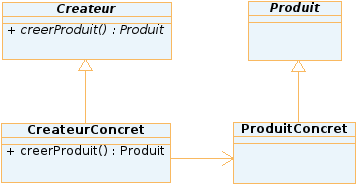
\includegraphics{fabrique.png}
\caption{Fabrique}
\label{fabrique}
\end{figure}


%Voici le diagramme des factory du jeu
\begin{figure}[H]
\center
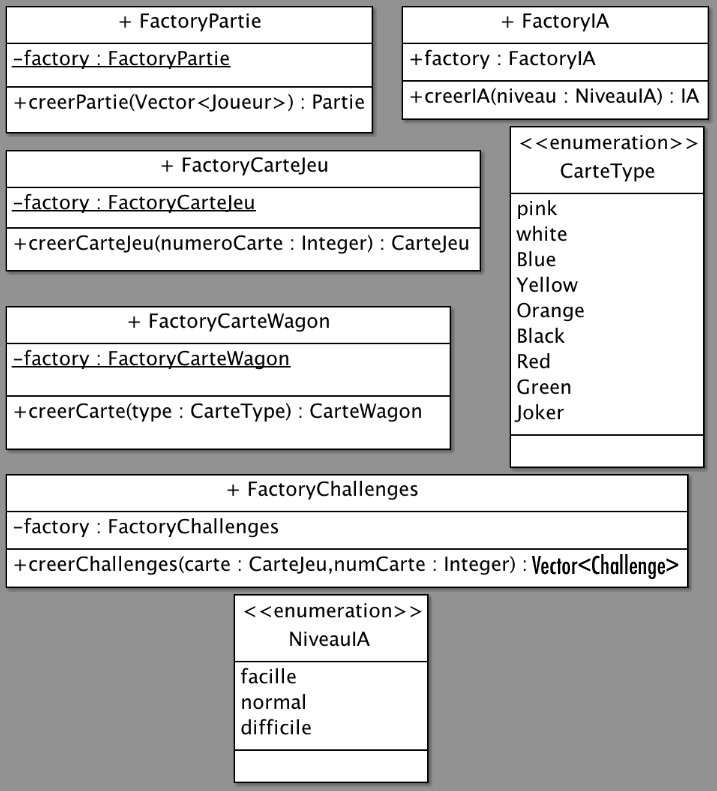
\includegraphics[width=400pt]{diagFactory.png}
\caption{Diagramme des factory}
\label{Factory}
\end{figure}
\subsubsection{FactoryPartie}
La FactoryPartie permet d'instancier une Partie en lui passant les joueurs de la partie, celle-ci instancie aussi les cartes wagons qui seront dans la partie. Elle fait donc appelle à la factory carte wagon en utilisant bien évidemment l'énumération CarteType qui représente les différentes cartes possibles dans le jeu.
\subsubsection{FactoryCarteJeu}
La FactoryCarteJeu permet d'instancier la carte et suivant le numéro passé en paramètre la carte est différente, c'est-à-dire que les UV et les routes ne seront pas les mêmes.\\
Cette factory permet donc d'avoir différentes carte de jeu et en plus de regrouper ce code, ça évite la duplication de code.
\subsubsection{FactoryCarteWagon}
La FactoryCarteWagon permet d'instancier des cartes wagons en passant en paramètre le type de la carte (CarteType).\\
De plus, comme expliqué plus loin, il est possible d'hériter de cette classe, de surcharger les méthodes et ainsi pouvoir ajouter de nouvelles cartes wagons.
\subsubsection{FactoryChallenges}
La FactoryChallenges permet de créer les challenges liés au numéro de carte passé en paramètre. La méthode renvoie un vector de challenges, il faut donc ensuite les ajouter à la partie qui est déjà instanciée.
\subsubsection{FactoryIA}
La FactoryIA permet de créer des joueurs qui vont être gérés par l'ordinateur, la difficulté de l'ia est liée au paramètre NiveauIA et de l'énumération des différents niveaux de l'IA.

\subsection{Conclusion du Pattern Factory et son utilité}
Grâce aux Factory le jeu reste ouvert (modulable) à la possibilté :
\begin{itemize}
\item de rajouter de nouvelles parties (nouvelles règles, ...)
\item d'ajouter de nouvelles cartes grâce au FactoryCarteJeu.\\La carte choisie est donnée grâce au "int numeroCarte" et le switch associé, de plus on peut hériter de cette factory et surcharger la méthode creerCarteJeu (utilisation de cette factory par exemple depuis un autre projet).
\item de créer de nouveaux challenges (liés à la carte). Les différents challenges sont instanciés suivant le numCarte passé en paramètre grâce au switch.
\end{itemize}


Par exemple, on peut si le jeu évolue ajouter de nouvelles carte wagon, il suffirait d'ajouter des lignes de codes dans FactoryCarteWagon (si on a accès à la source) sinon il suffit d'hériter de FactoryCarteWagon et d'instancier les nouvelles cartes et par défaut on appel la Factory mère ainsi on a surchargé la méthode mère pour créer des cartes.

\section{Des améliorations possibles}
\subsection{Ajouter des "achievements"}
Déjà possible avec la classe StatsSerializable (et Sauvegarde.java).\\
Il est aussi possible de créer des classes pour chaque achievement car il faut voir les achievement comme des classes qui héritent toutes d'une même classe abstraite "Achievement".
\subsection{Une meilleur définition d'une Partie}
Par amélioration d'une Partie, on veut dire qu'il aurait fallu créer une interface IPartie pour pouvoir bien définir les fonctions minimum d'une Partie, ceci aurait permis une aissance dans le fait de pouvoir hériter de la classe Partie et ainsi créer de nouvelles parties avec des règles différentes car les fonctions auraient été surchargées.


De plus avec cette interface on se serait plus rapproché de la manière dont a été pensé Slick2D, car si on étudie les sources de Slick2D on peut y voir beaucoup d'interface pour bien définir toutes les classes qui implémenteront ces interfaces (exemple: Game, InputListener, MouseListener, KeyListener, etc).


Les interfaces ne sont pas à n'égliger, elles permettent de bien définir les classes qui les implémente :
\begin{itemize}
\item \href{https://github.com/Blackdread/Drol2013/tree/master/src/base/engine/entities}{Exemple avec un ancien projet (et recréation des triggers,filter,etc du Source Engine)}  (https://github.com/Blackdread/Drol2013/tree/master/src/base/engine/entities)
\item \href{https://developer.valvesoftware.com/wiki/Source}{Wiki officiel du Source Engine}  (https://developer.valvesoftware.com/wiki/Source)
\end{itemize}
\subsection{Une gestion des erreurs personnalisées}
Il aurait fallu utilisé notre propre classe TicketUtbmExcpetion à la place de simple (err ou out) println.\\ Mais ce ne fût pas le cas quand on a commencé à programmer et on n'a donc pas fais cette classe.
\lstinputlisting[language=java, firstline=3, lastline=50, caption=Exception de Slick2D]{SlickException.java}

\chapter{Structure de la bibliothèque: Slick2D}\label{slick2dd}
Slick2D est une bibliothèque pour java qui permet la gestion des gui facilement et plus particulièrement pour créer des jeux vidéos en deux dimensions.
\section{Structure de base}
Tout projet Slick2D possède une base similaire :
\begin{itemize}
\item Une classe Game qui représente le jeux. Elle hérite de StateBasedGame.
Elle contient toutes les méthodes de bases d'un jeu. On hérite de cette
classe pour créer mon propre jeu.
\item Un AppGameContainer : C'est le conteneur du jeu. Une fois la classe Game instanciée, elle est passée en paramètre à cette classe qui implémente la boucle principale ( qui fait appel aux fonctions de la classe Game), qui gère les états (cf section sur le Game State Pattern \ref{gameStatePattern1} page \pageref{gameStatePattern1}).
\item Des états qui correspondent aux différentes vues du jeu (Menu principal, jeu, etc...)
\end{itemize}
Ainsi l'application instancie tout d'abord notre classe game auquel on a apporté nos modifications. Puis on a créé le conteneur en lui passant en paramètre notre Game. C'est en exécutant la fonction start() du conteneur que le programme est démarré, elle contient la boucle d'exécution.\\
C'est pourquoi nous allons d'abord nous pencher sur la boucle d'exécution principale.
\subsection{La boucle d'exécution principale}
La boucle d'exécution est déjà implémentée par Slick2D via la fonction start() du conteneur. Elle s'exécute de cette manière :
\begin{itemize}
\item Récupèrer le temps écoulé depuis le dernier tour de la boucle.
\item Gèrer les entrées clavier/souris.
\item Gèrer tout ce qui est lié au son.
\item Faire appel à la fonction update du jeu.
\item Faire appel à la fonction render du jeu.
\item Afficher la fenêtre openGL.
\end{itemize}
Ainsi nous n'avons pas à nous préoccuper de cette boucle, et seulement implémenter les méthodes d'update et de render de notre jeu. Leur appel sera automatiquement fait via ce conteneur. Cette abstraction permet de faciliter le développement.
\begin{lstlisting}[caption=La boucle principale : GameLoop()]
protected void gameLoop() throws SlickException {
		int delta = getDelta();
		if (!Display.isVisible() && updateOnlyOnVisible) {
			try { Thread.sleep(100); } catch (Exception e) {}
		} else {
			try {
				updateAndRender(delta);
			} catch (SlickException e) {
				Log.error(e);
				running = false;
				return;
			}
		}

		updateFPS();

		Display.update();
		
		if (Display.isCloseRequested()) {
			if (game.closeRequested()) {
				running = false;
			}
		}
	}
\end{lstlisting}

\begin{lstlisting}[caption=Update et render]
protected void updateAndRender(int delta) throws SlickException {
		//Pour avoir un "delta" arrondis
		if (smoothDeltas) {
			if (getFPS() != 0) {
				delta = 1000 / getFPS();
			}
		}
		// On gere les evenement ( Voir la classe Input de Slick2D )
		input.poll(width, height);
		//2) On gere la musique en prenant compte le temps ecoule
		Music.poll(delta);
		if (!paused) {
			storedDelta += delta;
			//Un temps suffisant s'est ecoule pour mettre a jour
			if (storedDelta >= minimumLogicInterval) {
				try {
					if (maximumLogicInterval != 0) {
						long cycles = storedDelta / maximumLogicInterval;
						for (int i=0;i<cycles;i++) {
							/*
							3) Mettre a jour le jeu autant de fois que le cycle
							a ete depasse (si le temps entre deux tour a ete long) */
							game.update(this, (int) maximumLogicInterval);
						}
						
						int remainder = (int) (delta % maximumLogicInterval);
						if (remainder > minimumLogicInterval) {
							game.update(this, (int) (delta % maximumLogicInterval));
							storedDelta = 0;
						} else {
							storedDelta = remainder;
						}
					} else {
						game.update(this, (int) storedDelta);
						storedDelta = 0;
					}
					
				} catch (Throwable e) {
					Log.error(e);
					throw new SlickException("Game.update() failure - check the game code.");
				}
			}
		} else {
			game.update(this, 0);
		}
		
		if (hasFocus() || getAlwaysRender()) {
			if (clearEachFrame) {
				// On efface la fenetre
				GL.glClear(SGL.GL_COLOR_BUFFER_BIT | SGL.GL_DEPTH_BUFFER_BIT);
			} 
			
			GL.glLoadIdentity();
			
			graphics.resetFont();
			graphics.resetLineWidth();
			graphics.setAntiAlias(false);
			try {
				//4) Rendu du jeu
				game.render(this, graphics);
			} catch (Throwable e) {
				Log.error(e);
				throw new SlickException("Game.render() failure - check the game code.");
			}
			graphics.resetTransform();
			
			if (showFPS) {
				defaultFont.drawString(10, 10, "FPS: "+recordedFPS);
			}
			//5) On affiche la fenetre open GL
			GL.flush();
		}
		
		if (targetFPS != -1) {
			Display.sync(targetFPS);
		}
	}
\end{lstlisting}

\section{Le Game State Pattern : machine à états}\label{gameStatePattern1}
En plus de gérer le conteneur, Slick2D procure un système d'état de jeu. Le jeu se trouve toujours dans un état précis qui correspond à une vue du jeu (menu principal, vue de chargement, etc...). Ces états sont représentés par la classe GameState. Cette classe nous procure les méthodes que toutes les vues (= état) possèdent :
\begin{itemize}
\item Enter qui permet l'exécution de tâches lorsque l'on rentre dans un état
\item Leave qui permet l'exécution de tâches lorsque l'on quitte un état
\item La gestion des évènements (mouse, keyboard, controller)
\item Render : Permet le rendu de l'état. On peut utiliser des méthodes faciles d'utilisation comme Draw qui permet de dessiner une image à un endroit donné.
\item Update : Permet de faire les mises à jour à chaque tour de boucle. Dans notre cas il fait appel à l'update d'une Partie.
\end{itemize}
Ainsi, notre classe game possède un état courant. Et lorsque le conteneur fait appel à la fonction update de notre clase game, elle exécute l'update de l'état. Le principe est similaire pour le render.

\chapter{La communication réseau}
\section{Principe général}
RPC (Remote Procedure Call) est un protocole réseau permettant de faire des appels de procédures sur un ordinateur distant à l'aide d'un serveur d'applications. Ce protocole est utilisé dans le modèle client-serveur pour assurer la communication entre le client, le serveur et des éventuels intermédiaires.
Un RPC est initié par le client qui envoie un message de requête à un serveur distant connu pour exécuter une procédure spécifique avec des paramètres spécifiques. Le serveur distant envoie une réponse au client et l'application continue son déroulement. Il y a beaucoup de variations et subtilités dans diverses implémentations, donnant lieu à une variété de différents protocoles RPC (incompatibles).\\
Exemple d'un protocol: Pendant que le serveur traite l'appel, le client est bloqué (il attend que le serveur ait terminé son traitement sur les données). Son inverse serait que le client n'attend pas de réponse du serveur et continue son exécution.
\subsection{Architecture du serveur/client}
Le serveur est hébergé chez une personne et les clients s'y connectent. Les actions des joueurs sont reçues sur le serveur et renvoyées aux joueurs.\\
La serialisation est bien évidemment utilisé pour communiquer et la connexion est faite en socket TCP.\\
Le jeu n'est pas simulé sur le serveur c'est donc les clients qui simulent tout, ce qui peut engendrer des désynchronisation lors d'évènement aléatoire c'est pourquoi il faut gérer ces cas rares en se fiant à un seul joueur ou écrire un algorithme qui cherche le résultat le plus "commun" parmis tous les joueurs et corriger chez ceux qui n'ont pas eu le même résultat.\\
Pour un diagramme de classes simple cf annexe \ref{network} page \pageref{network}.

\subsection{Implémentation}
La classe Server était à la base une classe pouvant acceptée plusieurs Partie en même temps, donc elle servait juste à faire la liaison entre les joueurs et leur partie. Dans le cadre de ce projet, cette classe a été simplifié pour n'accepter qu'une partie, on a toujours cette liaison serveur/client mais on n'a plus la possibilité de choisir la partie que l'on souhaite rejoindre.


La classe ClientServer permet au serveur de recevoir et gérer les différents clients qui se connectent. Il est donc possible d'affecter un ClientServer à une partie en particulier, ici on ne garde qu'une seule partie.


Les classes ThreadNetworkListener et ThreadNetworkSender sont les thread côté client qui permettent d'intéragir avec le serveur.
\chapter{Conclusion}
Ce projet a permis de mettre en place plusieurs notions vues en cours, TD et TP, et même d'aller plus loin (Factory, Game State Pattern, RPC, réseau, sauvegarde, sérialisation, etc).\\
De plus la réalisation du projet a permis de coder une architecture serveur/client en RPC, avec utilisation des socket. Ainsi on a pu utiliser nos connaissances et les approfondir.\\


En ce qui concerne le travail de groupe, un répertoire GitHub a été créé au début du projet pour faciliter le travail d'équipe.\\


Pour terminer, nous pensons avoir atteint les objectifs qui étaient fixés : 
\begin{itemize}
\item Interface
\item Code modulable
\item Modèle MVC
\item Adapter Ticket To Ride au monde de l'UTBM
\item Threads
\item Synchronisation\\
\end{itemize}


Il ne reste plus qu'à vous souhaiter bon jeu sur Ticket To UTBM.

\chapter{Logiciels utilisés}
\section{ArgoUML}
ArgoUML propose aux développeurs un outil de représentation UML, leader de la scène open source. L'application est compatible avec tous les diagrammes UML 1.4 standards et fonctionne sur n'importe quelle plateforme Java. ArgoUML est livré avec des profils pour le développement d'application C++ et Java. Il supporte les diagrammes de classe, les diagrammes d'état, les diagrammes "Use Case" ou encore les diagrammes de séquence, et plus encore. Enfin, ArgoUML offre des fichiers de sauvegarde ouverts basés sur du XML, et peut exporter les différents diagrammes aux formats GIF, PNG, PostScript, Encapsulated PS, PGML et SVG.
\begin{figure}[H]
\center

\includegraphics[width=70pt]{argoUML.png}
\caption{ArgoUML}
\label{ArgoUML}
\end{figure}
\section{Eclipse}
Eclipse  est  un  projet  de  la  Fondation  Eclipse  visant  à  développer  tout  un environnement de développement libre, extensible, universel et polyvalent. Je  l’ai  utilisé  pour  sa  facilité  d’utilisation  et  du  fait  que  c’est  un environnement de développement intégré (EDI).
\begin{figure}[H]
\center

\includegraphics[height=120pt]{eclipse.png}
\caption{Eclipse}
\label{Eclipse}
\end{figure}
\section{Java}
Le  projet  a  été  développé  en  java  langage  imposé  pour  sa  réalisation.  Le langage Java est un langage de programmation informatique orienté objet de Sun Microsystems.
\begin{figure}[H]
\center

\includegraphics[height=120pt]{java.png}
\caption{Java}
\label{Java}
\end{figure}
La  particularité  principale  de  Java  est  que  les  logiciels  écrits  dans  ce  langage sont  très  facilement  portables  sur  plusieurs  systèmes  d’exploitation  tels qu’UNIX, Windows, MacOS ou GNU/Linux, avec peu ou pas de modifications.

\appendix
\chapter{Documentation}
\section{Mes réalisations}
Voici une bonne partie de mes réalisations en programmation.
\\
\href{https://github.com/Blackdread/}{Mes réalisations sur GitHub} (https://github.com/Blackdread/)
\\

%Jeu réalisé lor du concours Innov'Game 2012
%\begin{itemize}
%\item \url{http://origins.dev.free.fr/}
%\item \url{http://originsdev.wordpress.com/}
%\item \url{http://08.innovgame.efrei.fr/}
%\end{itemize}
\section{Slick2D}
La bibliothèque graphique\\
\begin{itemize}
\item \href{http://slick.ninjacave.com/}{Site officiel} (http://slick.ninjacave.com/)
\item \href{https://bitbucket.org/kevglass/slick/src/9d7443ec33af/trunk/Slick/}{Code source de Slick2D}
\end{itemize}
\section{La réflexibilité / introspection}
\url{http://java.developpez.com/faq/java/?page=langage_reflexLado-}

\section{RMI}
\url{http://fr.wikipedia.org/wiki/Remote_method_invocation_(Java)}
\section{RPC}
C'est ce qui a été utilisé dans le projet. Toutes les actions du joueur sont envoyées au serveur (clique de la souris, touche appuyée,...)\\
\url{http://fr.wikipedia.org/wiki/Remote_procedure_call}

\chapter{Des exemples de code}
\label {StateBasedGame}
La classe StateBasedGame.java n'a pas été mise ici car beaucoup trop de ligne (prend 8 pages). Mais il est important d'aller voir cette classe pour comprendre un état dans Slick2D.\\



Tout simplement une classe qui permet de ne pas avoir à implémenter toutes les méthodes à chaque fois.
\lstinputlisting[language=java, caption=BasicGameState]{BasicGameState.java} \label {BasicGameState}


Un exemple d'une de mes vues, c'est la toute première vue du jeu on y charge toutes les ressources du jeu.
\label {exempleVue}
\begin{lstlisting}[caption=ResourcesView]
package lo43_TicketToRide.views;
// les import
/**
 * The second state of the game, a simple state to load resources. Like
 * presentation state this state load his own resources.
 * 
 * After loading all resources, the state move on the first view, the main menu
 * view.
 * 
 * @author Yoann CAPLAIN
 * 
 */
public class ResourcesView extends View {

	private static final int WAIT_TIME_BEFORE_NEXTR = 50;

	private boolean ready, doneOnce;
	private Image background;
	private ProgressBarFillRect bar;
	private Timer timer;

	private MouseOverArea butJouer, butRegle;
	
	private Rectangle rectFun;
	
	public ResourcesView(GameContainer container) {
		timer = new Timer(WAIT_TIME_BEFORE_NEXTR);
		this.container = container;
		initResources();
	}

	public void initResources() {
		ready=false;
		
		ResourceManager.addImage("western2", "western2.png");
		background = ResourceManager.getImage("western2");
		background = background.getScaledCopy(container.getWidth(), container.getHeight());
		
		// Init Music and Sounds
		GameMusic.initMainTheme();
		if(Configuration.isMusicOn()){
			GameMusic.setMusicVolume(Configuration.getMusicVolume());
			GameMusic.loopMainTheme();
		}
		
		ResourceManager.addImage("butJouer", "butJouer.png");
		ResourceManager.addImage("butJouerOver", "butJouerOver.png");
		ResourceManager.addImage("butRegle", "butRegle.png");
		ResourceManager.addImage("butRegleOver", "butRegleOver.png");
		
		Image tmp = ResourceManager.getImage("butJouer");
		
		int larg = tmp.getWidth();
		int haut = tmp.getHeight();
		
		int x = container.getWidth() / 2 - larg/2;
		int y = container.getHeight() / 2 - haut/2 * 4;
		
		butJouer = new MouseOverArea(container, tmp, x, y, larg, haut);
		butJouer.setMouseOverImage(ResourceManager.getImage("butJouerOver"));
		butJouer.setMouseDownSound(ResourceManager.getSound("butClick"));
		
		tmp = ResourceManager.getImage("butRegle");
		butRegle = new MouseOverArea(container, tmp, x, y+haut+10, larg, haut);
		butRegle.setMouseOverImage(ResourceManager.getImage("butRegleOver"));
		butRegle.setMouseDownSound(ResourceManager.getSound("butClick"));
		
		bar = new ProgressBarFillRect(2,8);
		bar.setLocation(container.getWidth() / 2 - 100, 3*container.getHeight() / 4);
		bar.setValue(40);
		
		rectFun = new Rectangle(10,100,50,20);
	}

	@Override
	public void render(GameContainer container, StateBasedGame sbGame, Graphics g) throws SlickException {
		super.render(container, sbGame, g);
		g.drawImage(background, 0, 0);
		if(!doneOnce){
			g.setColor(Color.red);
			bar.render(container, g);
			g.drawString("Loading ... " + ResourceManager.getAdvancement() + "%", bar.getX() + 20, bar.getY() - 25);
		}
		
		if (ready) {
			g.draw(rectFun);
			g.drawString("Ici", rectFun.getX()+5, rectFun.getY()+2);
			butJouer.render(container, g);
			butRegle.render(container, g);
		}	
	}

	@SuppressWarnings("static-access")
	@Override
	public void update(GameContainer container, StateBasedGame sbGame, int delta) throws SlickException {
		super.update(container, sbGame, delta);
		timer.update(delta);
		if (timer.isTimeComplete()) {
			ResourceManager.loadNextResource();
			if (ResourceManager.isLoadComplete() && !ready) {
				for (int i = 1; i < sbGame.getStateCount(); i++) {
					View view = ((Game) sbGame).getStateByIndex(i);
					view.initResources();
				}
				
				ready = true;
				
			}
			timer.resetTime();
		}
		if (bar != null)
			bar.setValue(((float) ResourceManager.getAdvancement()));
	}

	@Override
	public void keyPressed(int key, char c) {
		super.keyPressed(key, c);
		if(key == Input.KEY_ESCAPE)
			goToFun();
	}

	@Override
	public void mousePressed(int button, int x, int y) {
		super.mousePressed(button, x, y);
		if(butJouer.isMouseOver())
			goToMenuSolo();
		if(butRegle.isMouseOver())
			goToRegle();
		if(rectFun.contains(x, y))
			goToFun();
	}
	private void goToFun(){
		if (ready) {
		container.setMouseGrabbed(false);
		game.enterState(Game.FUN_VIEW_ID, new FadeOutTransition(), new FadeInTransition());
		}
	}
	private void goToRegle() {
		if (ready) {
			doneOnce = true;
			container.setMouseGrabbed(false);
			game.enterState(Game.REGLE_VIEW_ID, new FadeOutTransition(), new FadeInTransition());
		}
	}
	private void goToMenuSolo() {
		if (ready) {
			doneOnce = true;
			container.setMouseGrabbed(false);
			game.enterState(Game.MAIN_MENU_SOLO_VIEW_ID, new FadeOutTransition(), new FadeInTransition());
		}
	}
	@Override
	public int getID() {
		return Game.RESOURCES_STATE_ID;
	}

}
\end{lstlisting}

\chapter{Diagrammes}\label{Diagrammes}
Ce qui suit sont des diagrammes de classes plus simples mais qui représentent quasiment l'ensemble du projet.
\begin{figure}[H]
\center
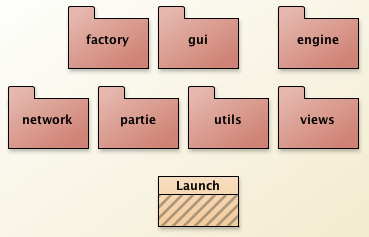
\includegraphics{launch.png}
\caption{launch}
\label{launch}
\end{figure}
\begin{figure}[H]
\center
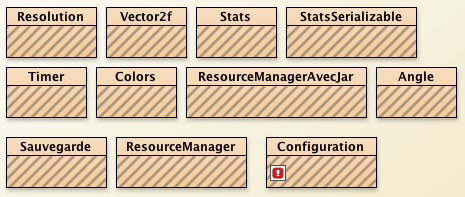
\includegraphics{utils.png}
\caption{utils}
\label{utils}
\end{figure}
\begin{figure}[H]
\center
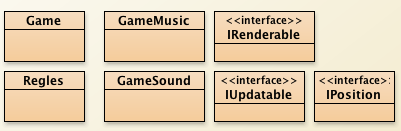
\includegraphics{engine.png}
\caption{engine}
\label{engine}
\end{figure}
\begin{figure}[H]
\center
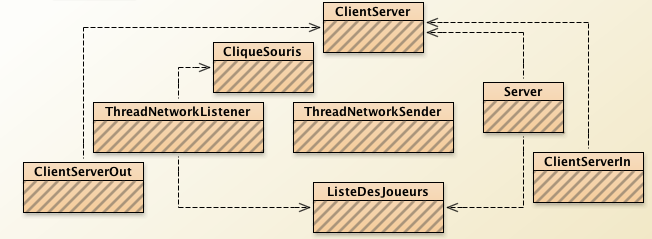
\includegraphics[width=400pt]{network.png}
\caption{network}
\label{network}
\end{figure}
\begin{figure}[H]
\center
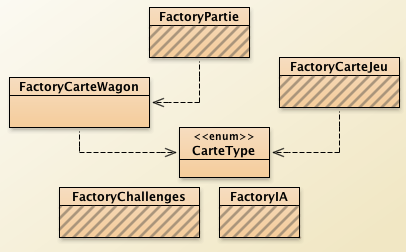
\includegraphics{factory.png}
\caption{factory}
\label{factory}
\end{figure}
\begin{figure}[H]
\center
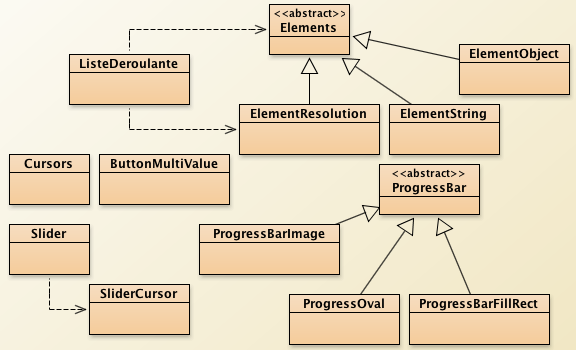
\includegraphics[width=480pt]{gui.png}
\caption{gui}
\label{gui}
\end{figure}
\begin{figure}[H]
\center
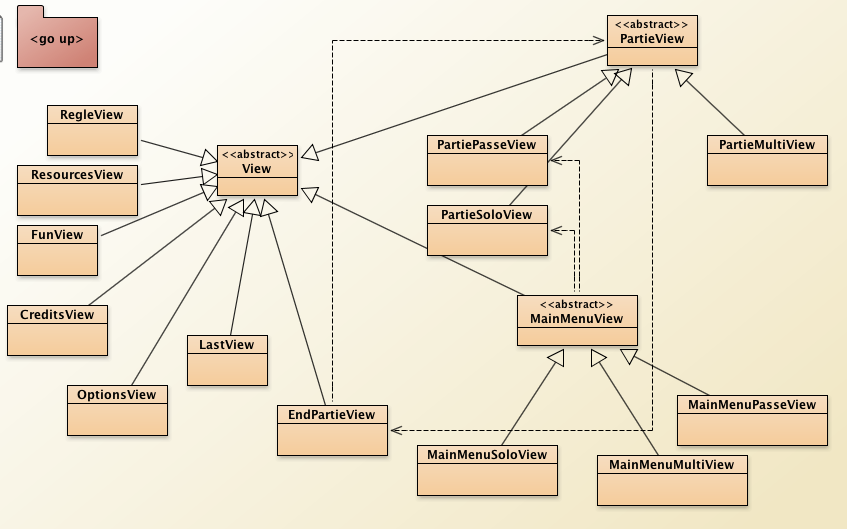
\includegraphics[angle=90,height=650pt]{views.png}
\caption{views}
\label{views}
\end{figure}
\begin{figure}[H]
\center
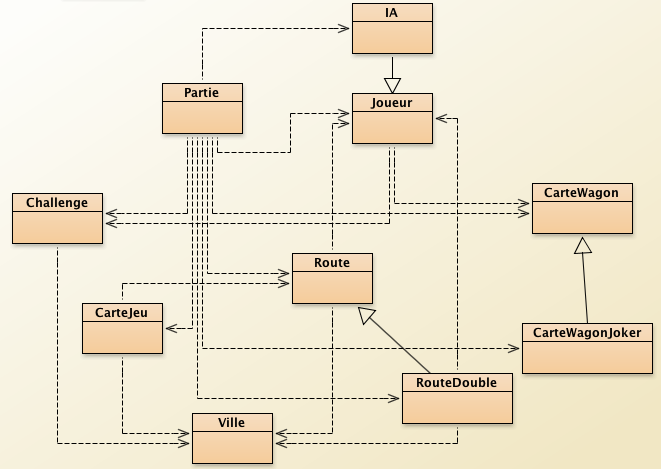
\includegraphics[angle=90]{partie.png}
\caption{partie}
\label{partie}
\end{figure}


\chapter{Images du jeu}
Quelques images de l'interface du jeu.
\begin{figure}[H]
\center
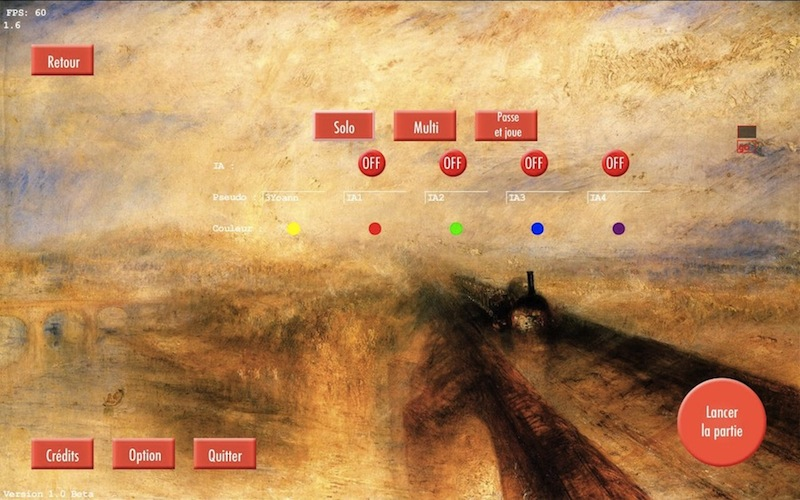
\includegraphics[width=500pt]{solo.jpg}
\caption{solo}
\label{solo}
\end{figure}
\begin{figure}[H]
\center
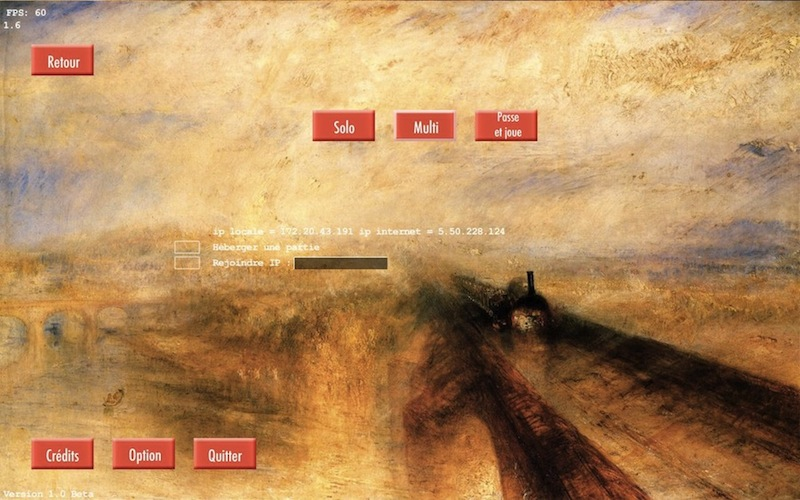
\includegraphics[width=500pt]{multi.jpg}
\caption{multi}
\label{multi}
\end{figure}
\begin{figure}[H]
\center
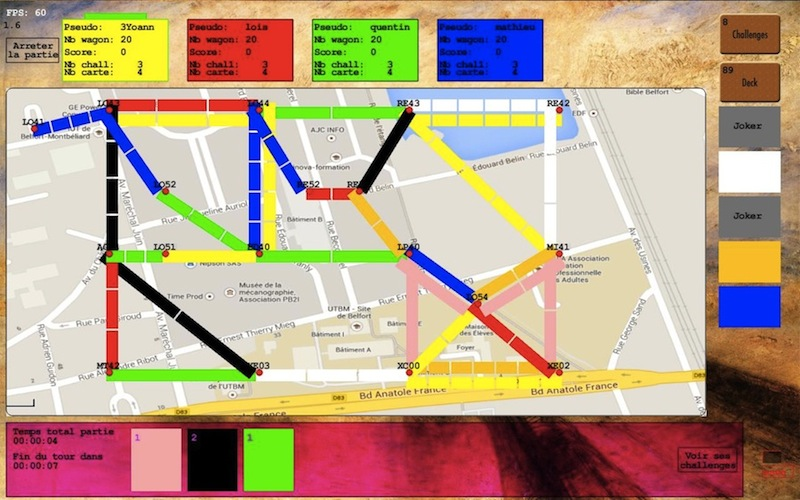
\includegraphics[width=450pt]{jeu1.jpg}
\caption{jeu1}
\label{jeu1}
\end{figure}
\begin{figure}[H]
\center
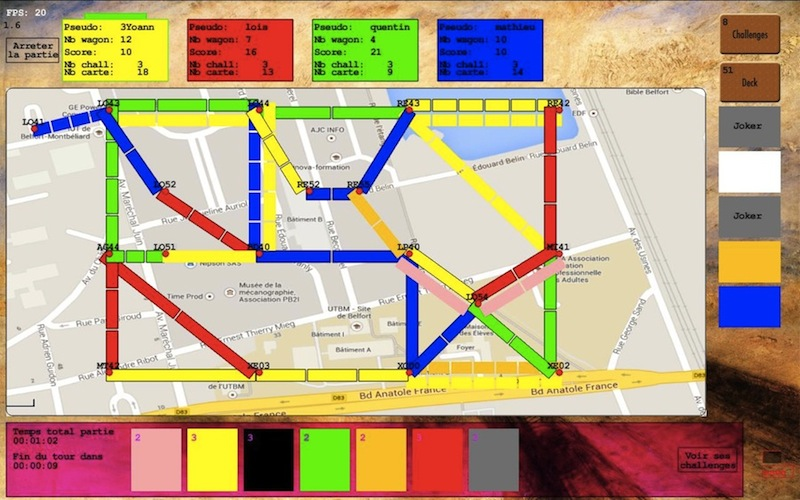
\includegraphics[width=450pt]{jeu2.jpg}
\caption{jeu2}
\label{jeu2}
\end{figure}
\end{document}